\begin{figure}[tb]
    \centering
    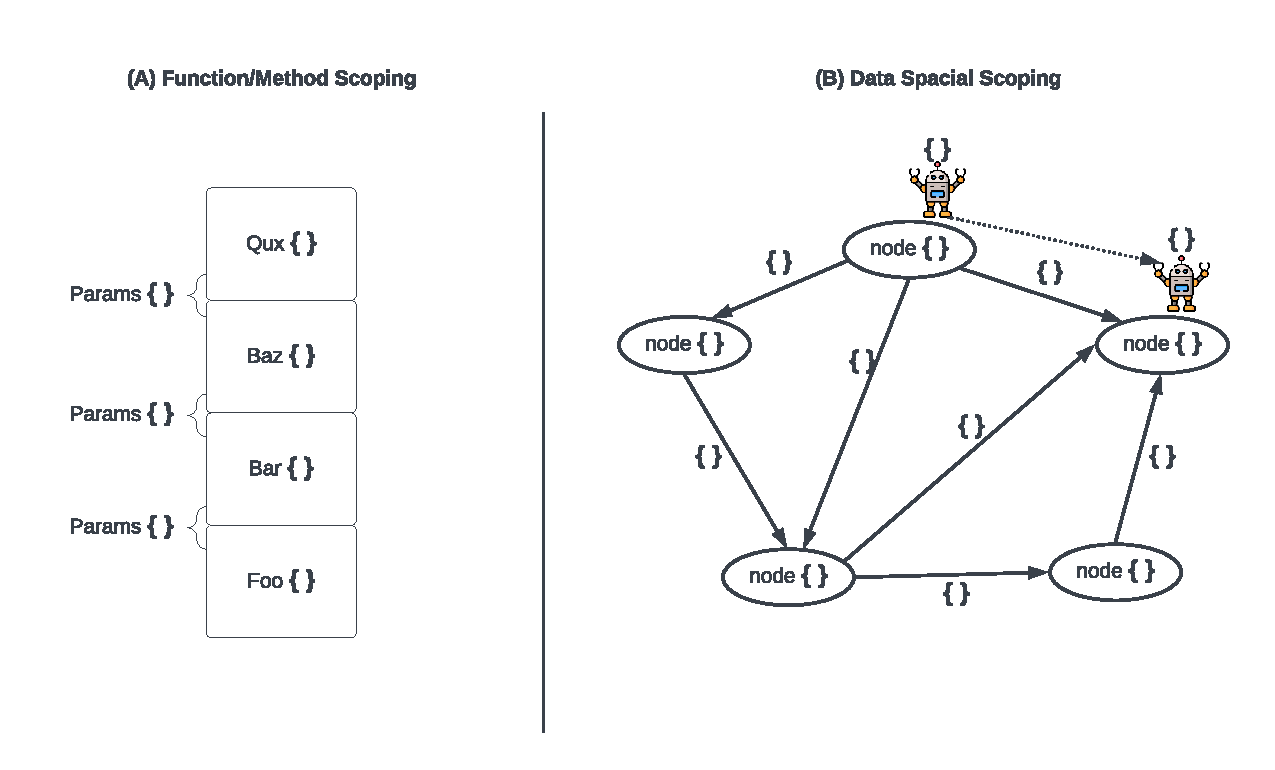
\includegraphics[width=\linewidth]{figures/data_spacial.pdf}
    \caption{A visualization of the behavior of scopes and problem solving abstractions provided by the near ubiquitous function / method based languages (left) and the data spacial programming model (right).}
    \label{fig:benefit}
\end{figure}

Traditionally in computer science, the task of raising the level abstraction in a computational model has primarily been for the goal of increasing programmer productivity.
This productivity comes from allowing engineers to function at the problem level while hiding the complexity of the underlying system.
The Jac language introduces a set of new abstractions guided by these principles based on two key insights.
First, Jac recognizes the emerging need for programmers to reason about and solve problems with graph representations of data.
Second, Jac further supports the need for algorithmic modularity and encapsulation to change and prototype production software in place of prior running codebases.
Based on these insights, we introduce two new sets of abstractions.
As shown in Figure~\ref{fig:benefit}b, Jac's \textbf{data-spacial scoping} natively facilitates graph based problem solving by replacing the traditional \emph{temporal} notion of scope with a function's activation record with scoping that is flattened and spatially laid out in graph structure.
This type of scoping allows for richer semantics for the organization of the data relevant to the problem being solved.
Figure~\ref{fig:benefit}b also depicts Jac's \textbf{agent oriented programming} as little robots.
Each robot carries scope with it as it walks and performs compute relevant to where it sits on the graph.
These `agent' abstractions capture the need for algorithmic modality and encapsulation when introducing solutions to already sophisticated codebases.
Jac can be used solely to build out complete solutions or as glue code with components built in other languages.
By leveraging these new language abstractions, HomeLendingPal~\cite{hlp-website} was able to create a production grade conversational AI experience with $\sim$300 lines of code in contrast to the tens of thousands it would take to build in a traditional programming language.